\section{Propuesta de Modelo}

\subsection{Dataset}
Se usará el FLAME dataset \cite{FLAME_Dataset} ya que este ha sido diseñado para estudios de
detección y segmentación de incendios, conteniendo imágenes y videos capturados mediante
drones en bosques del norte de Arizona. Para este proyecto, se usarán solo las imágenes y
se aprovechará que estas ya han sido distribuidas y etiquetadas para ser usadas:
39,375 imágenes para entrenamiento/validación y 8,617 imágenes para testeo.

\subsection{Arquitectura Propuesta}
Con el dataset de FLAME, se usará un ensamble de 3 modelos, los cuales serán: Xception,
DenseNet y ResNet; y posteriormente se destilarán en un modelo ligero como lo es
MobileNetV3. Además, se usarán ténicas de pruning antes del deployment para reducir
el tamaño del modelo y mejorar la eficiencia en la inferencia.

\begin{figure}[h]
    \centering
    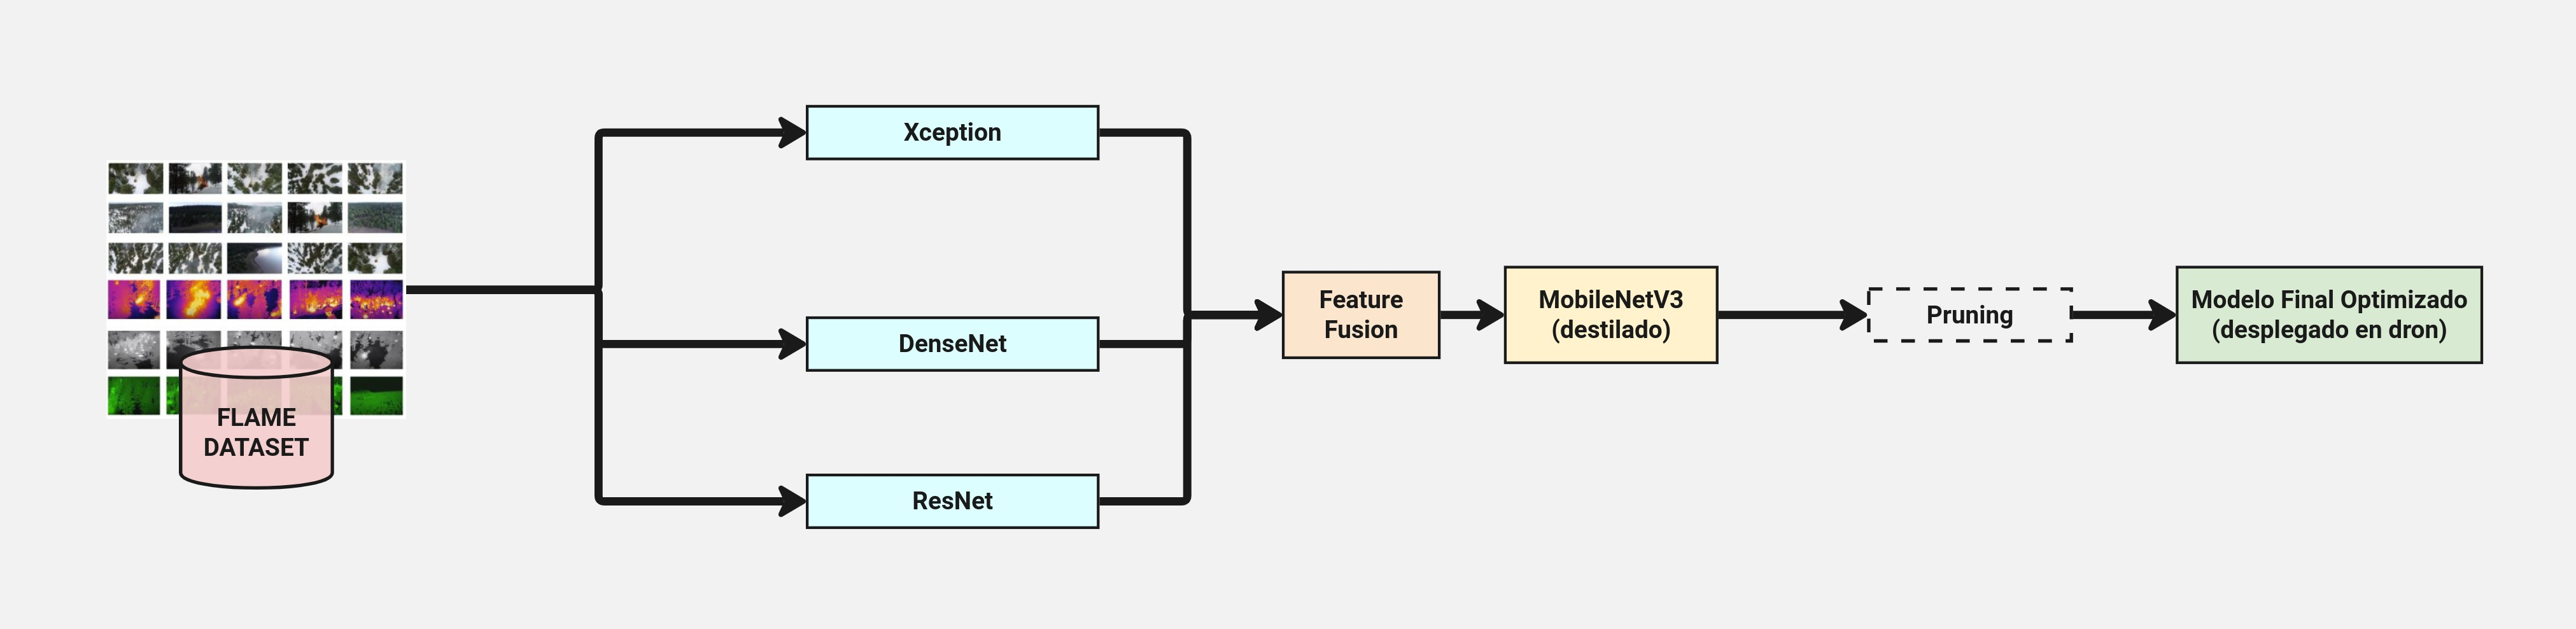
\includegraphics[width=0.9\textwidth]{images/model}
    \caption{Descripción del modelo}
    \label{fig:model}
\end{figure}

Se utilizarán \textbf{CNNs entrenadas sobre el dataset FLAME}, específicamente:

\begin{itemize}
    \item \textbf{Xception}: Utiliza \textit{Depthwise Separable Convolutions (DSC)} para optimizar la extracción de características, capturando relaciones complejas en la imagen. Se considera más eficiente en comparación con arquitecturas tradicionales.
    \item \textbf{DenseNet}: Usa \textit{bloques densos} que facilitan la reutilización de características, beneficiando la detección de elementos sutiles como \textit{ríos o humo de bajo contraste}.
    \item \textbf{ResNet}: Implementa \textit{conexiones residuales} para evitar la degradación del gradiente en redes profundas, lo que mejora la convergencia en entrenamientos largos.
\end{itemize}

\subsubsection{Entrenamiento previo al ensamble}
Cada modelo se entrenará \textbf{de manera individual} para la clasificación de incendios, empleando \textit{cross-entropy} como función de pérdida y aplicando \textit{early stopping} para evitar el sobreajuste.

\subsubsection{Fusión de Modelos (Ensamble)}
Una vez completados los entrenamientos individuales, se procederá con la fusión de modelos. Se consideran dos estrategias:

\begin{enumerate}
    \item \textbf{Fusión a nivel de salidas finales}:
    \begin{itemize}
        \item Se combinan las \textit{probabilidades} generadas por los tres modelos en un vector mayor.
        \item Se ajusta el \textit{peso} de cada modelo y se valida con \textit{cross-validation}.
    \end{itemize}

    \item \textbf{Fusión en capas intermedias}:
    \begin{itemize}
        \item Se extraen \textit{vectores de características} desde capas intermedias de cada modelo y se concatenan en un vector mayor.
        \item Se entrena un \textit{clasificador adicional} sobre este vector fusionado para generar la salida final.
    \end{itemize}
\end{enumerate}

\subsubsection{Knowledge Distillation}
Dado que el ensamble es \textbf{demasiado grande} para dispositivos con recursos limitados, se aplicará \textit{Knowledge Distillation}. Se entrenará un \textbf{MobileNetV3} como versión comprimida del ensamble, preservando la mayor cantidad de información relevante.

\subsubsection{Optimización Adicional: Pruning}
Para reducir aún más el tamaño del modelo, se aplicará \textit{pruning}, eliminando \textbf{pesos irrelevantes o de magnitud baja}. Esto permite reducir la carga computacional sin afectar significativamente la precisión.

\subsection{Justificación}

\begin{itemize}
    \item \textbf{Uso de Xception, DenseNet y ResNet en paralelo:}
    \begin{itemize}
        \item \textbf{Xception}: Usa convoluciones separables, reduciendo cálculos sin perder precisión.
        \item \textbf{DenseNet}: Mejora reutilización de características, ideal para detectar detalles pequeños.
        \item \textbf{ResNet}: Usa conexiones residuales, facilitando el entrenamiento en redes profundas.
    \end{itemize}
    \item \textbf{Destilación en MobileNetV3:}
    \begin{itemize}
        \item Modelo ligero y eficiente para \textit{drones}.
        \item Mantiene precisión al aprender de los modelos grandes.
    \end{itemize}
    \item \textbf{Ventajas sobre el estado del arte:}
    \begin{itemize}
        \item Más eficiente que ViT y ResNet en inferencia en dispositivos de bajo consumo.
        \item Mejor precisión que modelos CNN individuales.
    \end{itemize}
    \item \textbf{Despliegue en \textit{drones}:}
    \begin{itemize}
        \item Menor consumo de energía que ViT y CNNs pesados.
        \item Inferencia en tiempo real en \textit{Jetson Nano, Coral TPU, Raspberry Pi}.
    \end{itemize}
<<<<<<< HEAD
\end{itemize}
=======
\end{itemize}

\subsection{Pipeline}
El flujo de producción está diseñado para ejecutar una secuencia de cinco pasos que garantizan reproducibilidad y eficiencia. Estos pasos son:

\begin{enumerate}
    \item \textbf{Entrenamiento de DenseNet:} El modelo DenseNet se entrena utilizando hiperparámetros fijos y ajustados.
    \item \textbf{Entrenamiento de ResNet:} De manera similar, el modelo ResNet se entrena con sus mejores hiperparámetros.
    \item \textbf{Entrenamiento de Xception:} El modelo Xception se entrena bajo el mismo enfoque.
    \item \textbf{Ensamblado de modelos:} Las predicciones de los tres modelos entrenados se promedian para construir un modelo en ensamblado.
    \item \textbf{Destilación del modelo:} El modelo ensamblado actúa como maestro para destilar el conocimiento en un modelo estudiante más ligero.
\end{enumerate}

El script de bash (ubicado en \texttt{scripts/run\_pipeline.sh}) orquesta el flujo de trabajo.
>>>>>>> ae2c2836c37fe2e4b4ffbc943703ef797c84c406
